%----------------------------------------------------------------------------------------
%	PACKAGES AND THEMES
%----------------------------------------------------------------------------------------
\documentclass[aspectratio=169,xcolor=dvipsnames]{beamer}
\usetheme{Simple}

\usepackage{hyperref}
\usepackage{graphicx} % Allows including images
\usepackage{booktabs} % Allows the use of \toprule, \midrule and \bottomrule in tables
\usepackage{amssymb}
\usepackage{commath} % Align :=

\newcommand{\Go}{\mathbb{G}_0}
\newcommand{\Gi}{\mathbb{G}_1}
\newcommand{\Gt}{\mathbb{G}_T}
%----------------------------------------------------------------------------------------
%	TITLE PAGE
%----------------------------------------------------------------------------------------

% The title
\title[short title]{Algorand Community Study Group}
\subtitle{1: Elliptic Curve Cryptography}

\author[HMD2V] {HashMapsData2Value}
\institute[Algorand] % Your institution may be shorthand to save space
{
    % Your institution for the title page
    Digital Community Champion \\
    Algorand Foundation \\
    \vskip 3pt
}
\date{\today} % Date, can be changed to a custom date


%----------------------------------------------------------------------------------------
%	PRESENTATION SLIDES
%----------------------------------------------------------------------------------------

\begin{document}

\begin{frame}
    % Print the title page as the first slide
    \titlepage
\end{frame}


\begin{frame}{Welcome!}
\begin{itemize}
    \item Welcome!
    \item Study group? Discord: \href{https://discordapp.com/channels/491256308461207573/1092424979091566622}{\#cryptography-study-group}
    \item GitHub Repo: \href{https://github.com/HashMapsData2Value/Algorand-Community-Study-Group/tree/main/Topics}{https://github.com/HashMapsData2Value/Algorand-Community-Study-Group}
    \item Please introduce yourselves
    \item Topic - Elliptic Curve Cryptography
    \item Chapter 15 in \textit{A Graduate Course in Applied Cryptography} by Dan Boneh and Victor Shoup (version 0.6)
\end{itemize}
\end{frame}

\begin{frame}{Agenda}
    % Throughout your presentation, if you choose to use \section{} and \subsection{} commands, these will automatically be printed on this slide as an overview of your presentation
    \tableofcontents
\end{frame}

\section{Chapter 15}

\subsection{15.1 The group of points of an elliptic curve}
    \begin{frame}{15.1 The group of points of an elliptic curve}

    \begin{columns}[c] % The "c" option specifies centered vertical alignment while the "t" option is used for top vertical alignment

    \column{.55\textwidth} % Left column and width
        \begin{itemize}
            \item Diophantus, $y^2 = x^3 - x + 9$ (Rational)
            \item Points: (x,y)
            \item Chord Method, $U \boxplus V = - W$, $U \neq -V$
            \item Tangent Method, $P \boxplus P = Q$, $y \neq 0$
        \end{itemize}


    \column{.5\textwidth} % Right column and width
    \begin{figure}
        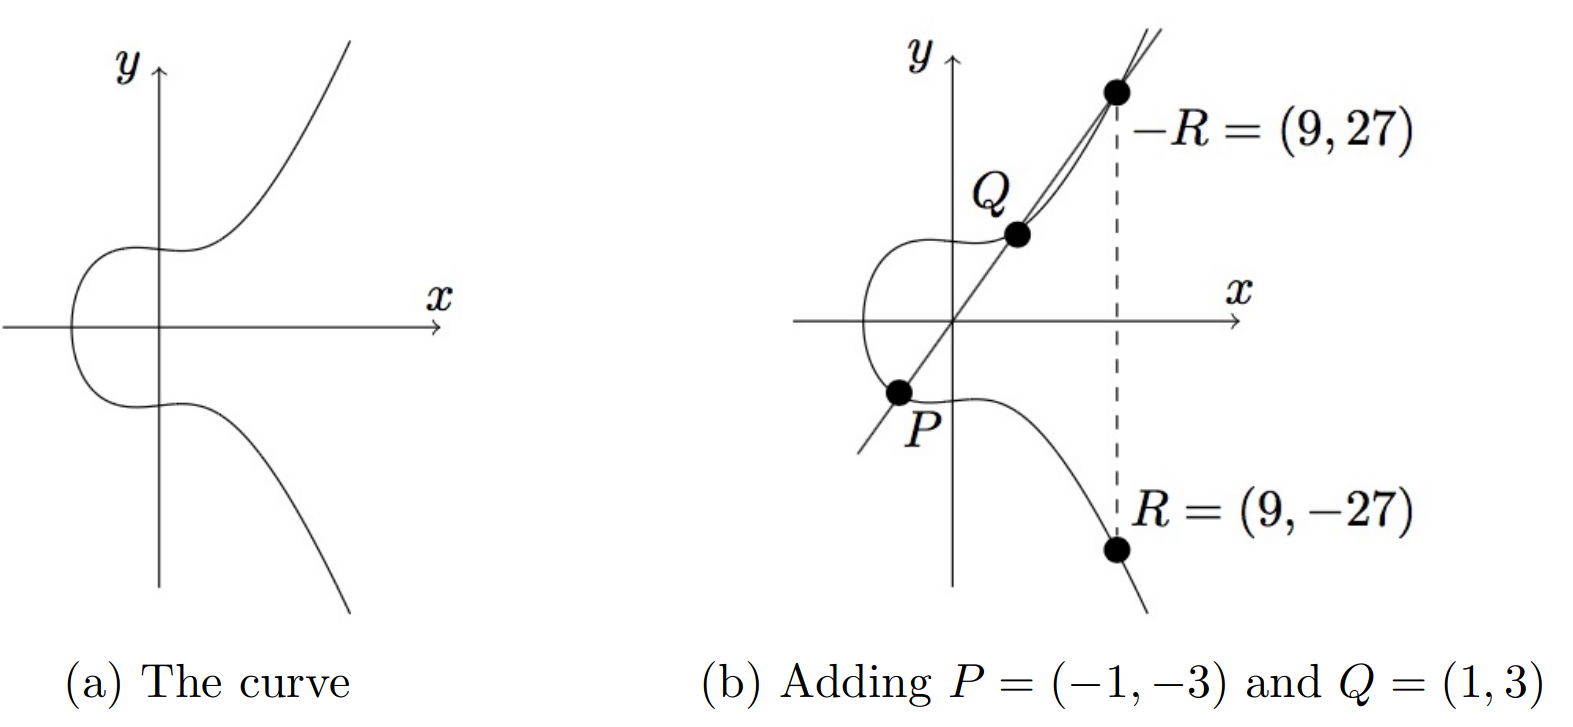
\includegraphics[width=1\linewidth]{Figure15.1.png}
    \caption{Credits \cite{p1}.}
    \end{figure}
    \end{columns}

\end{frame}

\subsection{15.2 Elliptic curves over finite fields}
    \begin{frame}{15.2 Elliptic curves over finite fields}
        \begin{itemize}
            \item Rationals $\mathbb{Q}$ ($1, 4.2, \frac{9}{36}, -3$) $\rightarrow$ Finite Field $\mathbb{F}$ ($..., -1, 0, 1, 2, ... \mod{p}$) $\mathbb{Z}/p\mathbb{Z}$
            \item $E/\mathbb{F}_p$ - denotes elliptic curve defined over finite field 
            \item $E(\mathbb{F}_{p^e})$ - denotes the set of all points on curve + the "point at infinity $\mathbb{O}$"
            \item Example: $E$: $y^2 = x^3 + 1$, $p = 11$ $\rightarrow$ $E(\mathbb{F}_{11}) = \{ \mathbb{O}, (-1, 0), (0, \pm 1), (9, \pm 2), (6, \pm 3), (8, \pm 4), (3, \pm 5)  \}$
            \item $|E(\mathbb{F}_{11})| = 12$ "group elements"
            \item Group Operation - $\boxplus$. $\mathbb{O}$ is identity element $P \boxplus \mathbb{O} = P$
            \item Pick one point to be a "generator"! Will generate a group of certain order.
            \item Two notations: $\underbrace{G + G + ... + G}_\text{a additions} = A$, $\underbrace{g*g*...* g}_\text{a multiplications} = g^a$.
            \item Forms: Weierstrass, Edward, Montgomery 
        \end{itemize}
\end{frame}

\subsection{15.3 Elliptic curve cryptography}
    \begin{frame}{15.3 Elliptic curve cryptography}
    \begin{itemize}
        \item Let $G, g \in E(\mathbb{F}_{p^e})$ of order $q$ (i.e. generates group of $q$ number points on curve). If $q$ is itself prime, then:
        \begin{itemize}
            \item $qG \equiv \mathbb{O}$ (additive) or $g^q \equiv \mathbb{O}$ (multiplicative)
            \item Discrete Log Problem: $\alpha G \equiv A \rightarrow \alpha \equiv A/G$ or $g^\alpha \equiv a \rightarrow \alpha \equiv log(a)_g$ HARD!
        \end{itemize}
        \item Need to be careful! You're in trouble if:
        \begin{itemize}
            \item $|E(\mathbb{F}_p)| = p$, i.e. there are as many unique points on the curve as we have integers in our finite field, or
            \item There exists a small integer $\tau$ such that $|E(\mathbb{F}_p)|$ divides $p^\tau - 1$.
        \end{itemize}
    \item So we just stick to standard curves and parameters, e.g:
    \begin{itemize}
        \item P256 - Shady! NSA didn't explain a certain parameter...
        \item Curve25519 - Algorand!
        \begin{itemize}
            \item Ed25519, refer to explanation in the \href{https://github.com/HashMapsData2Value/Algorand-Community-Study-Group/blob/main/Topics/1. Elliptic Curve Cryptography/HMD2V Notes.md}{repo notes under \#ed25519-signature}.
            \item With signatures: scalar $\alpha$ is secret key, $\alpha G = A$ is public key. Secret key signs transactions from public key (address).
        \end{itemize}
    \end{itemize}
    \end{itemize}
    \end{frame}
    
\subsection{15.4 Pairing based cryptography}
    \begin{frame}{15.4 Pairing based cryptography - Definition}
    \begin{theorem}[Definition 15.2. in \cite{p1}]
        Let $\Go, \Gi, \Gt$ be three cyclic groups of prime order q where $g_0 \in \Go$ and $g_1 \in \Gi$ are generators. A pairing is an efficiently computable function $e : \Go \times \Gi \rightarrow \Gt$ satisfying the following properties:
        \begin{enumerate}
            \item bilinear: for all $u, u^{'} \in \Go$ and $v, v^{'} \in \Gi$ we have
            \begin{enumerate}
                \item $e(u \cdot u^{'}, v) = e(u,v) \cdot e(u^{'}, v)$, and
                \item $e(u, v \cdot v^{'}) = e(u,v) \cdot e(u, v^{'})$
            \end{enumerate}
            \item non-degenerate: $g_T := e(g_0, g_1)$ is a generator of $\Gt$ (and doesn't just output $1 \in \Gt$ for all inputs) 
            
        \end{enumerate}
    \end{theorem}
    \begin{itemize}
        \item If $\Go = \Gi$ pairing is "symmetric", otherwise asymmetric. $\Go$ and $\Gi$ are called the "pairing groups" and $\Gt$ the target group.
        \item (Obviously) we construct pairings from elliptic curves.
    \end{itemize}
    \end{frame}
    \begin{frame}{15.4 Pairing based cryptography - Groups}
        \begin{itemize}
            \item $\Go$ is order $q$ subgroup of $E(\mathbb{F}_p)$, for some prime $q$.
            \item $\Gi$ is order $q$ subgroup of $E(\mathbb{F}_{p^d})$, for some $d > 0$ (embedding degree of curve) where $\Gi \cap \Go = \{\mathbb{O}\}$
            \item $\Gt$ is an order $q$ multiplicative subgroup of the finite field $\mathbb{F}_{p^d}$.
            \item Note that as $\Go$ is defined over base field $\mathbb{F}_p$ and $\Gi$ over a larger field $\mathbb{F}_{p^d}$ points in $\Go$ are "smaller" We want $d$ to be not too large as we'd get a huge $\Gi$. $d < 16$ is "pairing friendly".
            \item Central property: $e(g_{0}^{\alpha}, g_{1}^{\beta}) = e(g_0, g_1)^{\alpha \cdot \beta} = e(g_{0}^{\beta}, g_{1}^{\alpha})$
            \item Pairing function $e$ - Weil pairing (variant: Tate and Ate pairings), efficiently evaluated with Miller's algorithm.
        \end{itemize}
    \end{frame}

    \begin{frame}{15.4 Pairing based cryptography - DDH}
        \begin{itemize}
            \item Pairings were originally thought to be BAD! Why?
            \item When $\Go = \Gi$ decision Diffie-Hellman (DDH) problem in $\Go$ no longer HARD
            \item DDH: For $\alpha, \beta, \delta \overset{{\scriptscriptstyle\$}}{\leftarrow} \mathbb{F}_p$ (secret) and $g_{0}^\gamma = g_{0}^{\alpha * \beta}$, $g_{0}^\delta$ and $g_{0}^\gamma$ both look "random". I.e. shouldn't be possible for an "outsider" to decide whether  $\delta$ or $\gamma$ $ = \alpha * \beta$...
            \item However, $e(g_{0}^\alpha, g_{0}^\beta) \overset{?}{=} e(g_{0}, g_{0}^\gamma) \rightarrow e(g_0, g_0)^{\alpha * \beta} = e(g_0, g_0)^\gamma$
            \item (Note: Not to be confused with $\gamma = \alpha + \beta$ as checking $g^\gamma = g^\alpha * g^\beta = g^{\alpha + \beta}$ is trivial.
            \item This makes e.g. ElGamal encryption scheme insecure on $\Go$.
            \item For $\Go \neq \Gi$ asymmetric pairings DDH assumption might hold in both $\Go$ and $\Gi$. It does for "the most efficient asymmetric pairings".
            \item Also, we need to pick groups that ensure discrete log problem is HARD in $\Gt$, otherwise it breaks down in $\Go$ and $\Gi$. ($u := e(g_{0}^\alpha, g_1) = e(g_0, g_1)^\alpha = g_{T}^\alpha$. If $\alpha = log(u)_{g_T}$ easy...)
        \end{itemize}   
    \end{frame}

\begin{frame}{15.4 Pairing based cryptography - Curves}
      \begin{table}
        \begin{tabular}{l c c c c c c}
            \toprule
            \textbf{name} & \textbf{$d$} & \textbf{$q$ group order} & \textbf{$\mathbb{F}_p$ size} & \textbf{$\Go$ bytes} & \textbf{$\Gi$ bytes} & \textbf{advantage}  \\
            \midrule
            bn256 & 12 & 256 & 256   & 32    & 64    & Speed     \\
            bls381 & 12 & 256 & 381   & 48    & 96    & Security \\
            \bottomrule
        \end{tabular}
        \caption{Comparison between curves bn256 and bls381. They are also called BN254 and BLS 12-381 respectively, e.g. in AVM docs}
    \end{table}

    \begin{itemize}
        \item bn256 faster due to smaller finite field it is defined over, while bls381 more secure as the DLOG problem in $\Gt$ is harder.
    \end{itemize}
\end{frame}

\begin{frame}{15.4 Pairing based cryptography - Speed Tricks}
    \begin{itemize}
        \item Exponentiation in $\Go$ fastest (0.22 ms), then $\Gi$ (0.44 ms), then $\Gt$ (0.95 ms). Pairing $\Go \times \Gi \rightarrow \Gt$ (2.32 ms). 
        \item $e(g_{0}^\alpha, g_{1}) = e(g_{0}, g_{1}^\alpha) = e(g_{0}, g_{1})^\alpha$ - same results, different computation speeds.
        \item A product of pairings $\prod^{n}_{i=1}e(u_{i}, v_{i}) \in \Gt$ can also be sped up by aggregating final exponentiation. E.g $n=3$:
        \begin{itemize}
            \item $u_1, u_2, u_3 \in \Go \rightarrow g_{0}^\alpha, g_{0}^\beta, g_{0}^\gamma$
            \item $v_1, v_2, v_3 \in \Gi \rightarrow g_{1}^\delta, g_{1}^\epsilon, g_{1}^\zeta$
            \item $e(g_{0}^\alpha, g_{1}^\delta)e(g_{0}^\beta, g_{1}^\epsilon)e(g_{0}^\gamma, g_{1}^\zeta) =e(g_0, g_1)^{\alpha \delta}e(g_0, g_1)^{\beta \epsilon}e(g_0, g_1)^{\gamma \zeta} = e(g_0, g_1)^{\alpha \delta + \beta \epsilon + \gamma \zeta}$
        \end{itemize}
        \item (Provides intuition for how Groth16 ZK-SNARKs are so efficient.)
    \end{itemize}
\end{frame}

\subsection{Intermission: AVM EC Math Pull Request}
\begin{frame}{AVM EC Math Pull Request}
\begin{itemize}
    \item \href{https://github.com/algorand/go-algorand/pull/4924}{https://github.com/algorand/go-algorand/pull/4924} (Liable to change!)
    \item New opcodes (each with option for BN254 or BLS318, $\Go$ or $\Gi$):
    \begin{itemize}
        \item ec\_add: $A + B = C, \in \mathbb{G}$ (equivalent to $g^a * g^b = g^c$)
        \item ec\_scalar\_mul: $\alpha P = A \in \mathbb{G}$ (equivalent to $(g)^a$)
        \item ec\_multi\_exp: multiple inputs version of ec\_scalar\_mul.
        \item ec\_pairing\_check: Check if $e(A_1, B_1)e(A_2, B_2)...e(A_n, B_n) = 1$.
        \item ec\_subgroup\_check: check if point is "valid" ($\in \mathbb{G}$)
        \item ec\_map\_to: maps input to point (i.e., $H(m) \in \mathbb{G}$)
    \end{itemize}
    \item Pairing check VERY expensive, only possible in logic sig (stateless smart contract)
\end{itemize}
    
\end{frame}

\subsection{15.5 Signature schemes from pairings}

\begin{frame}{15.5 Signature schemes from pairings - BLS}
\begin{theorem}[Boneh-Lynn-Shacham (BLS) Signature Scheme]
    BLS algorithms:
    \begin{itemize}
        \item Key Generation: $sk := \alpha \overset{{\scriptscriptstyle\$}}{\leftarrow} \mathbb{Z}_{q}, pk := g_{1}^{\alpha} \in \Gi$. 
        \item Sig. Generation: $\sigma \leftarrow H(m)^\alpha \in \Go$
        \item Sig. Verification: $e(H(m), pk) \overset{?}{=} e(\sigma, g_1)$
    \end{itemize}
\end{theorem}
    \begin{itemize}
        \item Hash function $H: \mathbf{M} \rightarrow \Go$ (maps input directly to $\Go$, a point.)
        \item Signature $\sigma$ a point in $\Go$, $pk$ a point in $\Gi$.
        \item  $e(H(m), pk) = e(H(m), g_{1}^\alpha) = e(H(m)^\alpha, g_1) = e(\sigma, g_1)$
    \end{itemize} 
\end{frame}

\begin{frame}{15.5 Signature Schemes from pairings - BLS Advantages}
\begin{itemize}
    \item Since $\sigma \in \Go$, the signature is short (32 bytes for bn256)!
    \begin{itemize}
        \item Compare with 64 bytes signatures in Ed25519, though without expensive pairing operation.
        \item BLS possible to swap s.t. $pk \in \Go$ and $\sigma \in \Gi$ - short public key instead. 
    \end{itemize}
    \item BLS applications:
    \begin{itemize}
        \item Signature Aggregation
        \begin{itemize}
            \item Verify many signatures with few operations
        \end{itemize}
        \item Threshold Signatures
        \begin{itemize}
            \item $t$ out of $n$ signers are enough to sign message 
        \end{itemize}
        \item Blind Signatures
        \begin{itemize}
            \item Signer signs encrypted message, but message integrity verifiable.
        \end{itemize}
        \item Distributive generation of secret key across several parties
    \end{itemize}
\end{itemize}
\end{frame}

\begin{frame}{15.5.2 Signature Aggregation}
\begin{theorem}[BLS Signature Aggregation]
    Given $\textbf{pk} = (pk_1, ..., pk_n) \in \Gi^n$, messages $\textbf{m} = (m_1, ..., m_n)$ and signatures $\boldsymbol{\sigma} = (\sigma_1, ..., \sigma_n) \in \Go^n$, we have the following algorithms:
    \begin{itemize}
        \item Gen. Sig. Aggregate: $\sigma_1 * \sigma_2 * ... * \sigma_n \rightarrow \sigma_{ag}$ (short)
        \item Ver. Sig. Aggregate: $e(\sigma_{ag}, g_1) = e(H(m_1), pk_1)*...*e(H(m_n), pk_n)$
    \end{itemize}
\end{theorem}
\begin{itemize}
    \item $e(\sigma_{ag}, g_1) = e(\sigma_1 * ... * \sigma_n, g_1) = \prod^{n}_{i=1} e(\sigma_i, g_1) = \prod^{n}_{i=1} e(H(m_i)^{\alpha}_{i}, g_1) = \prod^{n}_{i=1} e(H(m_i), g_1^{\alpha}_{i}) = \prod^{n}_{i=1} e(H(m_i), pk_{i})$
    \item Remember: aggregation doesn't have to be "one-time" process, it can happen gradually.
    \item If $m_1 = m_2 = ... = m_n$ (single message) $e(\sigma_{ag}, g_1) = e(H(m), apk), apk := pk_1 * ... * pk_n$. $apk$ is an aggregate public key, can be pre-computed.
\end{itemize}
\end{frame}

\begin{frame}{15.5.2 Signature Aggregation - Rogue Key}
    \begin{alertblock}{WARNING: Rogue Key Attack!}
    BLS signature aggregation scheme works but is susceptible to rogue key attack, where an adversary targeting Bob can maliciously create a key that "negates" other keys in the aggregated signature.

    The adversary can make it seem like Bob signed something he actually did not.

    Thus, if you decide to implement BLS signature aggregation you must use one of two methods to make it secure:
    \begin{itemize}
        \item Message Augmentation
        \item Proof of Possession of Secret Key
    \end{itemize}
\end{alertblock}
\end{frame}

\subsection{15.6 Advanced encryption schemes from pairings}
\begin{frame}{15.6 Advanced encryption schemes from pairings - IBE}
\begin{block}{Identity-based Encryption (IBE)}
"An Identity Base Encryption (IBE) scheme is a public-key cryptosystem where any string is a valid public key. In particular, email addresses and dates can be public keys." - \href{https://crypto.stanford.edu/ibe/}{Stanford}
\end{block}
\begin{itemize}
    \item Requires "Private Key Generator" (PKG), trusted coordinator with master secret key. With $msk$ you can decrypt everything, but possible to distribute it across multiple parties.
    \item Advantages?
    \begin{itemize}
        \item Saves DB space! (We already store usernames!)
        \item Expiration: $pk := $ user@email.com $||$ [today]. (New secret key every day!)
        \item Delegation: e.g. use email subject line as $pk$, different labels $\rightarrow$ different decryption keys, given to different people.
    \end{itemize}
    \item Paper: BasicIdent - \cite{p2}.
\end{itemize}
\end{frame}

\subsection{15.7 The functional encryption paradigm}
\begin{frame}{15.7 The functional encryption paradigm - Levels}
\begin{itemize}
    \item Basic level: 1 key pair for encryption/decryption. All or nothing.
    \item Next level: (IBE) 1 master key pair + encrypt/decrypt by ID key pair
    \item Can we GENERALIZE this and obtain a broad definition of public-key encryption?
    \begin{itemize}
        \item $(pk, msk) \leftarrow Setup(1^\lambda)$ - creates public key and master secret key.
        \item $sk_f \leftarrow KeyGen(msk, f)$ - generates functional $sk_f$ for a function $f$ using $msk$.
        \item $c \leftarrow Enc(pk, m)$ - uses $pk$ to encrypt input $x$.
        \item $y \leftarrow Dec(sk_f,c)$ - uses $sk_f$ to calculate $y = f(x)$.
    \end{itemize}
    \item In fact... 
    \begin{itemize}
        \item For "basic", $f$ is identity function $I$. $msk = sk_f$ (only one functional $sk$), and it decrypts any well-formed ciphertext.  
        \item For IBE, there is a $sk_{id'}$ for every $id' \in ID$. $c$ can be decrypted by $sk_{id'}$ if $c$ was encrypted against $id'$.
    \end{itemize}
\end{itemize}
\end{frame}

\begin{frame}{15.7 The functional encryption paradigm - Examples}
\begin{itemize}
    \item Linear functional encryption
    \begin{itemize}
        \item Doesn't strictly require pairings...
        \item Allows for linear fitting on encrypted data, e.g. medical data.
        \item Can give access to specific subset of points.
    \end{itemize}
    \item Quadratic functional encryption
    \begin{itemize}
        \item Allows for calculating variance and standard deviation on encrypted data.
    \end{itemize}
    \item Attribute-based encryption
    \begin{itemize}
        \item Instead of polynomials, predicate functions: $f: x \rightarrow \{0, 1\}$ (and families of a set of them).
        \item Ciphertext $c = (x,m)$ - an encryption of attribute $x$ and message $m$.
        \item Decryption is dependent on the secret key matching the attribute of the data (predicate function gives 1).
    \end{itemize}
\end{itemize}
    
\end{frame}

\subsection{15.8 Multilinear Maps}
\begin{frame}{15.8 Multilinear Maps}
\begin{itemize}
    \item Bilinearity is \textit{really} nice. Wouldn't it be nice if we could get multilinearity?
    \begin{itemize}
        \item $e(g_{0}^{\alpha_0}, g_{1}^{\alpha_1}, ..., g_{n}^{\alpha_n}) = e(g_0, g_1, ..., g_n)^{\prod^{n}_{i=0} \alpha_i}$
        \item ($g_T := e(g, ..., g)$ a generator of $\Gt$.) 
    \end{itemize}
    \item Active field of research...
    \item Example application: Secret Sharing (you're the $\alpha$)
    \begin{itemize}
        \item 2 parties: $g^\alpha$, $g^\beta \rightarrow (g^\beta)^\alpha = g^{\alpha \beta}$
        \item 3 parties: $g^\alpha, g^\beta, g^\gamma \rightarrow e(g^\beta, g^\gamma)^\alpha = e(g,g)^{\alpha \beta \gamma} =  g{_T}^{\alpha \beta \gamma}$
        \item 4 parties: [No \textit{practical} solution....]
    \end{itemize}
\end{itemize}
\end{frame}

\begin{frame}{Anything else?}
    \Huge{\centerline{Did we forget something?}}
\end{frame}

\section{Next topic?}
\begin{frame}{Next topic?}
\begin{itemize}
    \item The Smörgåsbord of inspiration: 
    \begin{itemize}
        \item Lattice-based Cryptography (State Proofs/FALCON Keys, Learning with Errors, FHE?)
        \item Monero's Tech (Ring Signatures, Bulletproofs, ...)
        \item ZK-SNARKs (Groth16, PLONK, ...)
        \item Casino games with hidden state (IOHK-sponsored Royale, Kaleidoscope, 21; ZK proof of correctness of shuffles...)
        \item Algorand Foundation's research into SMPC (SPRINT, TCaaS, NI-PVSS)
    \end{itemize}
    \item Anything else?
    \item We can decide details on Discord...
\end{itemize}
    
\end{frame}
%-------------------------------------------- TEMPLATE!



\begin{frame}{References}
    % Beamer does not support BibTeX so references must be inserted manually as below
    \footnotesize{
        \begin{thebibliography}{99}
            \bibitem[Boneh, Shoup, 2023]{p1} Dan Boneh and Victor Shoup (2023 v0.6)
            \newblock A Graduate Course in Applied Cryptography
            \newblock \emph{cryptobook.us} 15, 615 -- 681.
            \bibitem[Boneh, Frankin]{p2} Dan Boneh and Matthew Franklin (2003)
            \newblock Identity based encryption from the Weil pairing
            \newblock \emph{SIAM J. of Computing} Vol. 32, No. 3, pp. 586-615, 2003 
        \end{thebibliography}
    }
\end{frame}

%------------------------------------------------

\begin{frame}
    \Huge{\centerline{The End (for now!)}}
\end{frame}

%----------------------------------------------------------------------------------------

\end{document}